\subsection{Discussion}\label{sec:discussion}
\newcommand{\baselineEvalFigure}{
\begin{figure}[t]
    \centering
    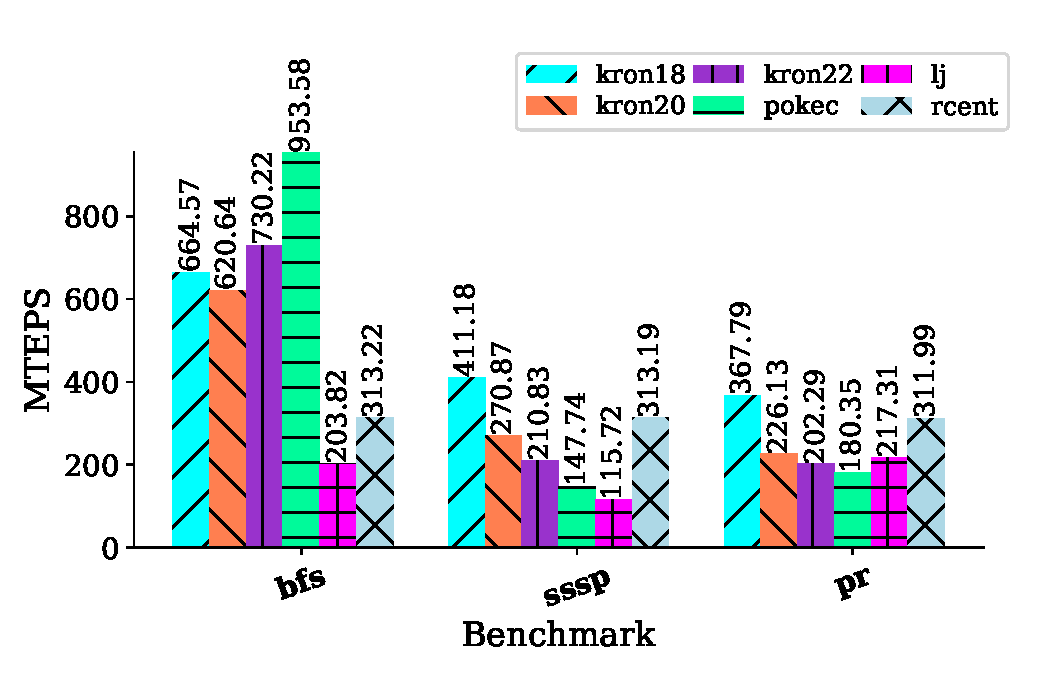
\includegraphics[scale = 0.5]{graphit-figures/baseline.pdf}
    \caption{Baseline code generation results for each benchmark in the dense pull direction with no manycore specific optimizations.}
    \label{pap:generals:sec:eval:fig:baseline}
\end{figure}
}

\newcommand{\pushEvalFigure}{
\begin{figure}[t]
    \centering
    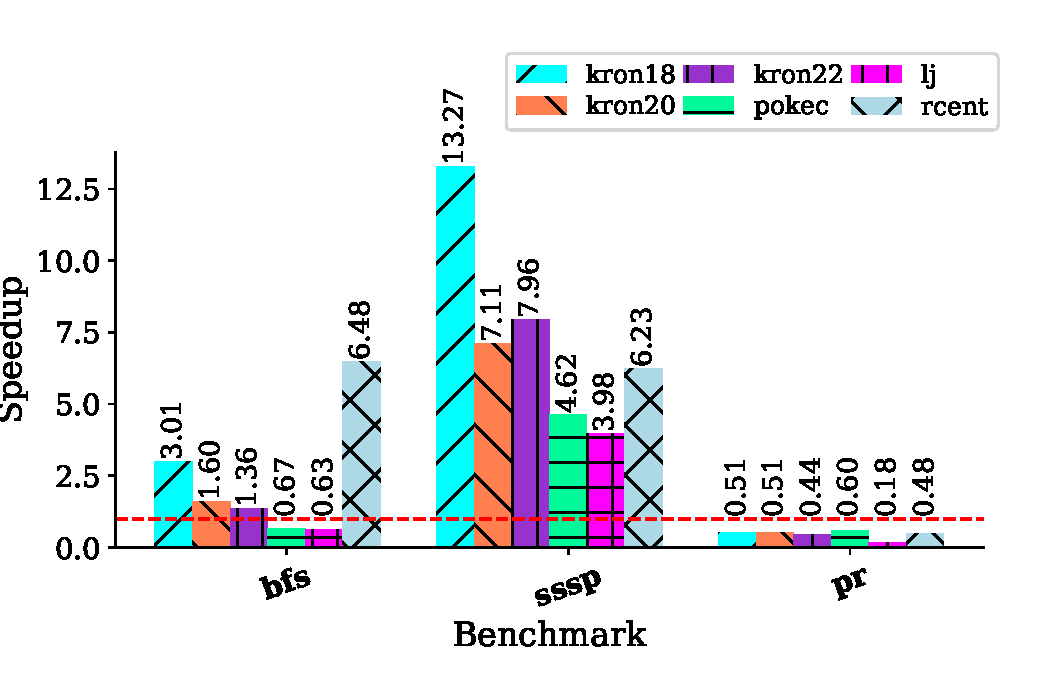
\includegraphics[scale = 0.5]{graphit-figures/push.pdf}
    \caption{Baseline code generation results for each benchmark in the push direction with no manycore specific optimizations.}
    \label{pap:generals:sec:eval:fig:push}
\end{figure}
}

\newcommand{\edgeSpeedupFigure}{
\begin{figure}[t]
    \centering
    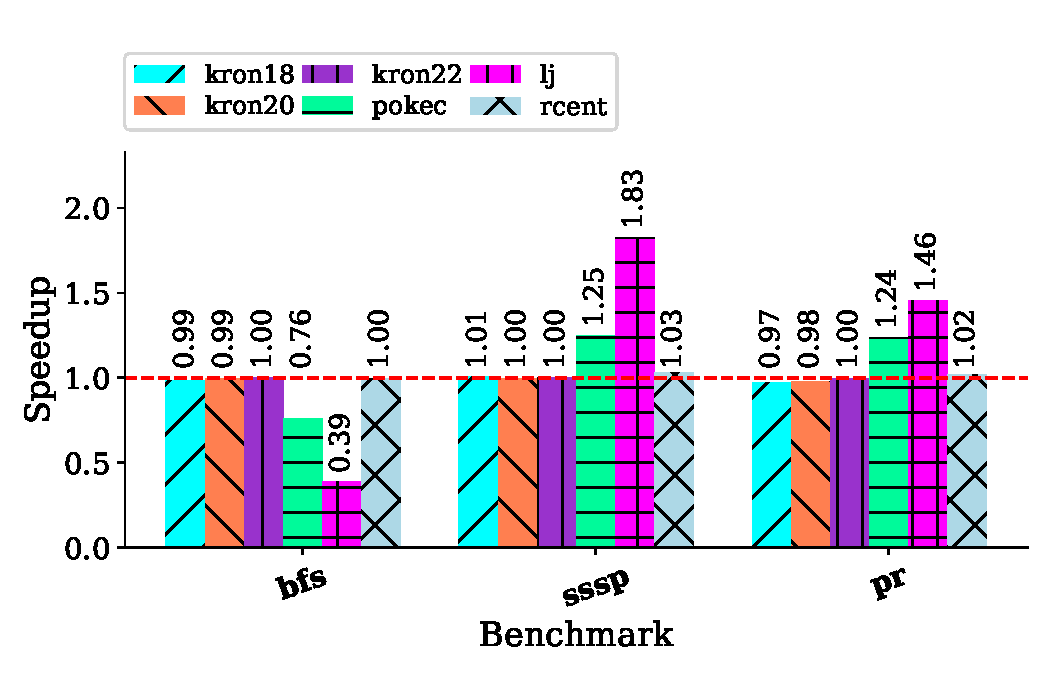
\includegraphics[scale = 0.5]{graphit-figures/edge.pdf}
    \caption{Speedup results for edge based optimization over the baseline dense pull implementation for each benchmark.}
    \label{pap:generals:sec:eval:fig:edge}
    \vspace{-2mm} 
\end{figure}
}

\newcommand{\blockBFSFigure}{
\begin{figure}[t]
    \centering
    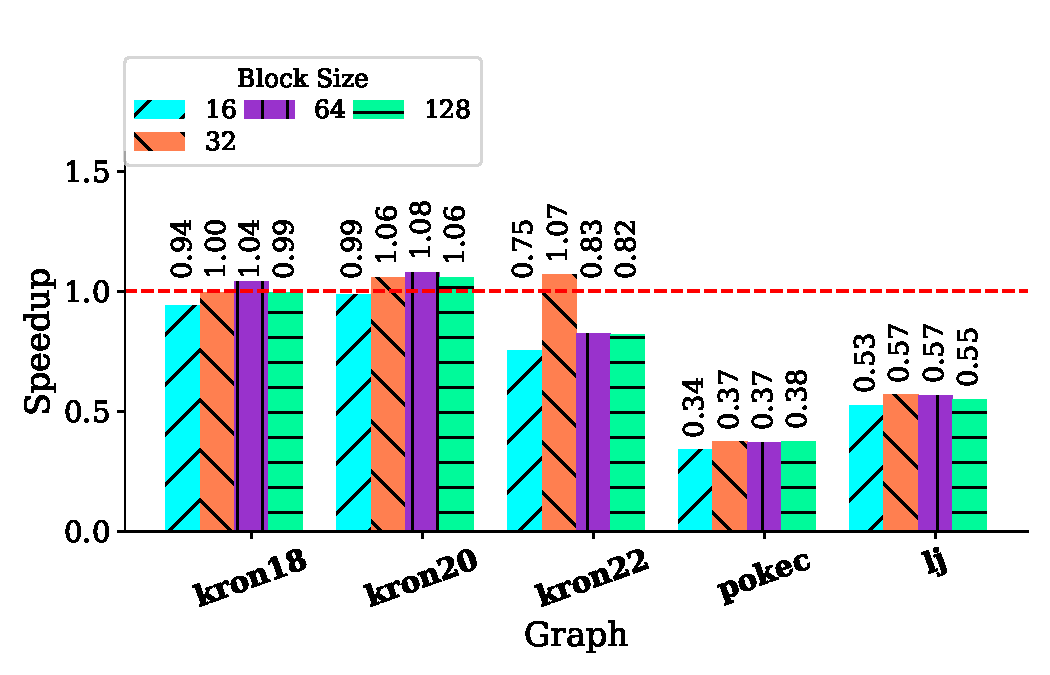
\includegraphics[scale = 0.5]{graphit-figures/bfs-block.pdf}
    \caption{MTEPS results for varying block sizes using the blocked access method on BFS.}
    \label{pap:generals:sec:eval:fig:bfsblock}
\end{figure}
}

\newcommand{\blockSSSPFigure}{
\begin{figure}[t]
    \centering
    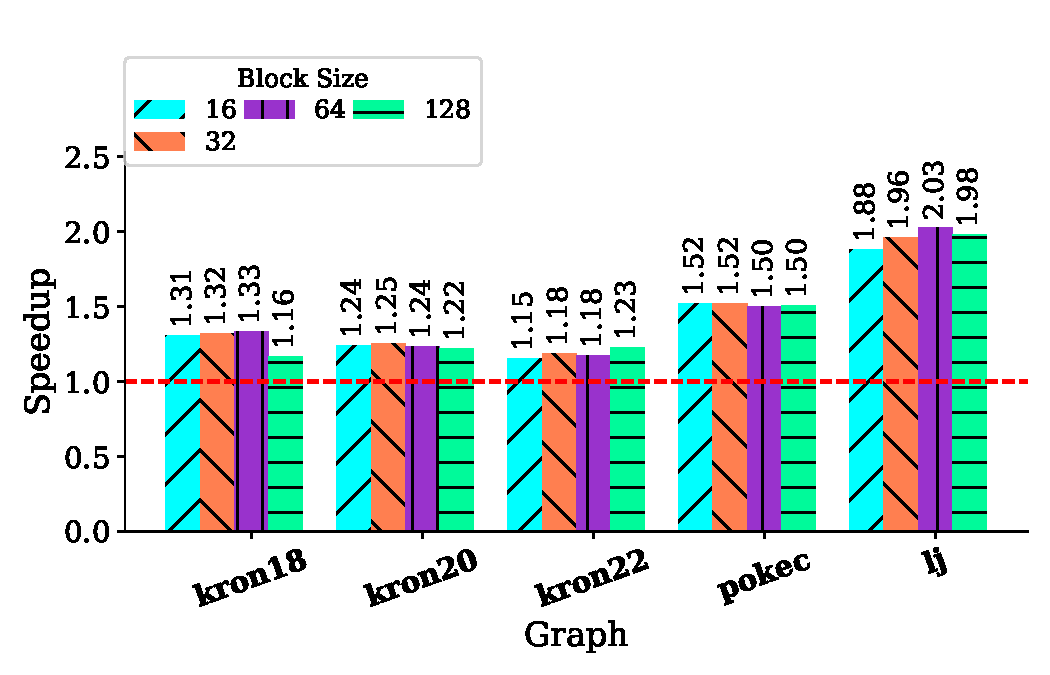
\includegraphics[scale=0.5]{graphit-figures/sssp-block.pdf}
    \caption{Speedup results for varying block sizes using the blocked access method on SSSP. Speedup is calculated over the baseline pull direction implementation.}
    \label{pap:generals:sec:eval:fig:ssspblock}
\end{figure}
}

\newcommand{\cacheBFSFigure}{
\begin{figure}[t]
    \centering
    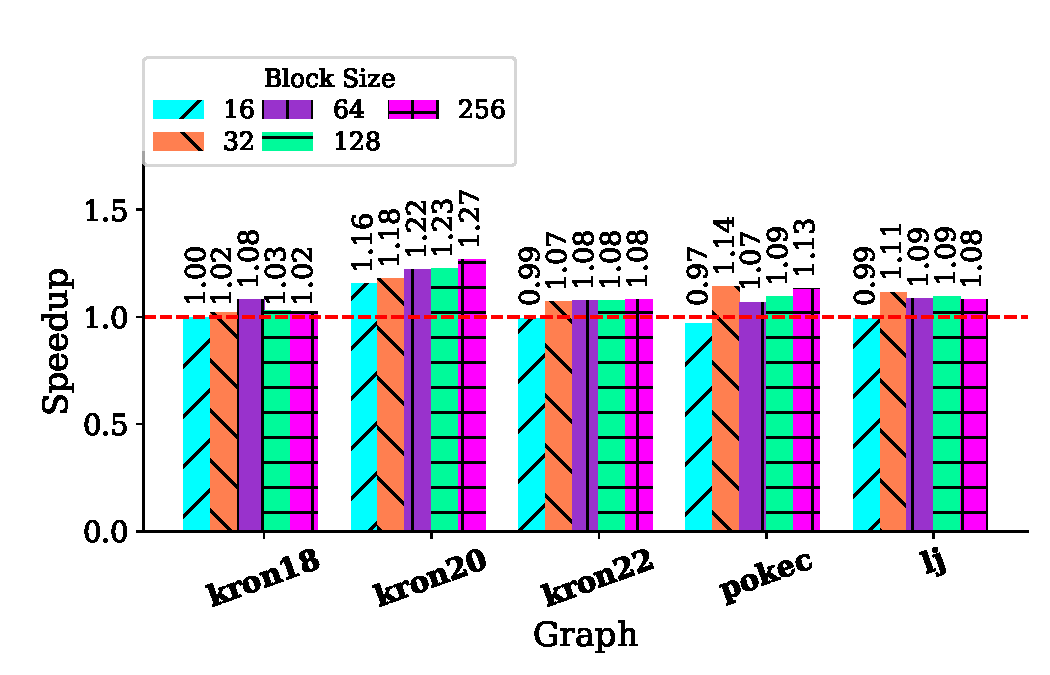
\includegraphics[scale = 0.5]{graphit-figures/bfs-cache.pdf}
    \caption{MTEPS results for varying work block sizes using the manycore aware vertex partitioning scheme on BFS.}
    \label{pap:generals:sec:eval:fig:bfscache}
\end{figure}
}

\newcommand{\cacheSSSPFigure}{
\begin{figure}[t]
    \centering
    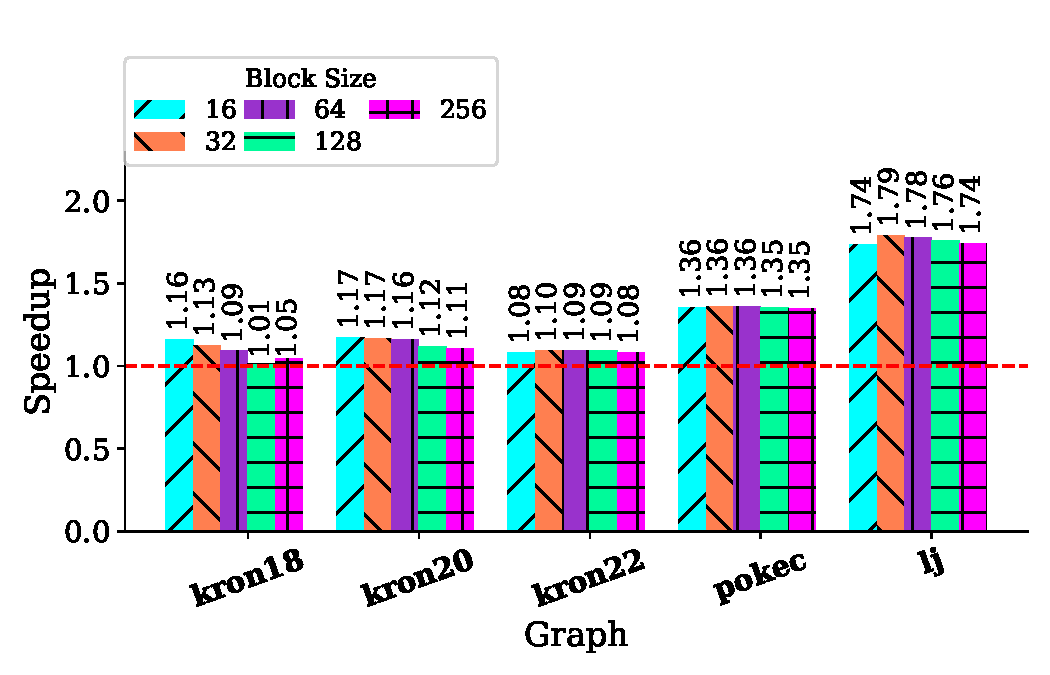
\includegraphics[scale=0.5]{graphit-figures/sssp-cache.pdf}
    \caption{Speedup results for varying work block sizes using the manycore aware vertex partitioning scheme on SSSP. Speedup is calculated over the baseline pull direction implementation.}
    \label{pap:generals:sec:eval:fig:ssspcache}
\end{figure}
}

\newcommand{\allBlockedFigure}{
\begin{figure}[t]
    \centering
    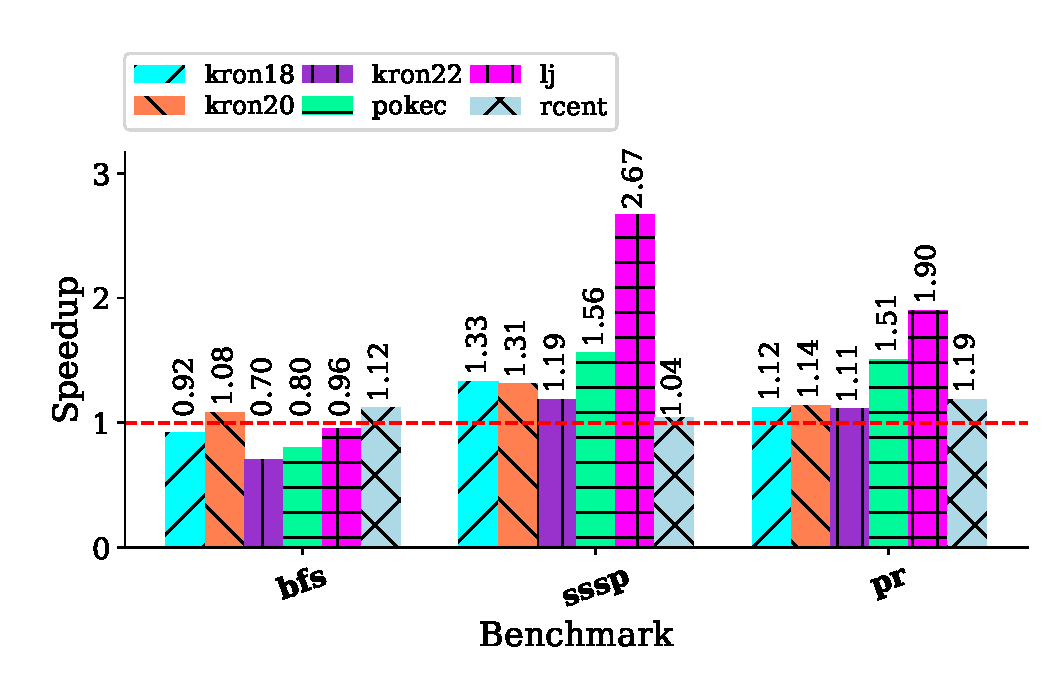
\includegraphics[scale = 0.5]{graphit-figures/all-blocked.pdf}
    \caption{Blocked access method speedup results for each benchmark. Speedup is calculated over the baseline pull direction implementation.} %For each graph and benchmark, block sizes of 16, 32, 64, and 128 elements were tested and the best performing block size is reported here.
    \label{pap:generals:sec:eval:fig:blocked}
\end{figure}
}

\newcommand{\allAlignedFigure}{
\begin{figure}[t]
    \centering
    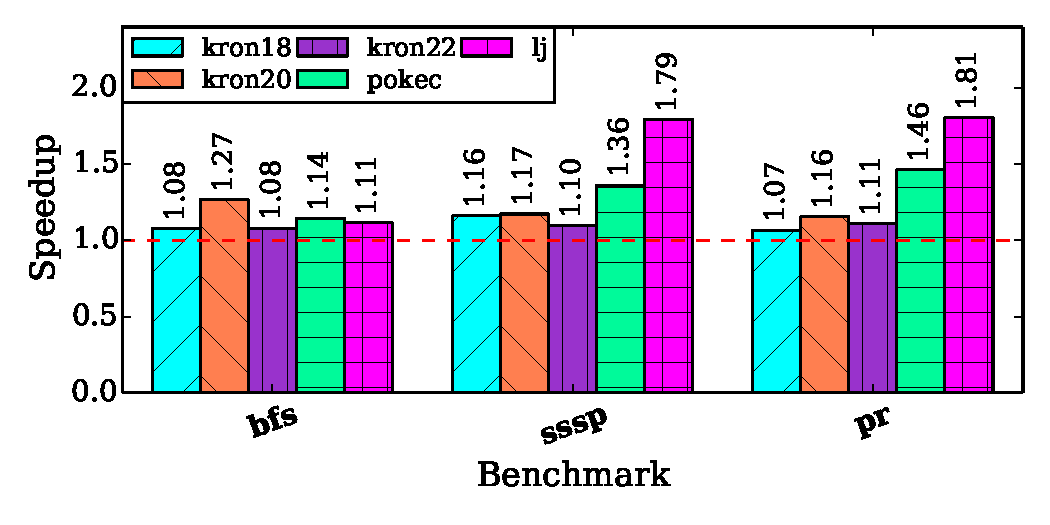
\includegraphics[scale = 0.5]{graphit-figures/align.pdf}
    \caption{Alignment-based partitioning speedup results for each benchmark. Speedup is calculated over the baseline pull direction implementation.} %For each graph and benchmark, work group sizes of 16, 32, 64, 128, and 256 vertices were tested and the best performing work group size is reported here.
    \label{pap:generals:sec:eval:fig:aligned}
    \vspace{-2mm} 
\end{figure}
}

%I am not sure if this is the best way to present an overview of results or if we need it. 
\newcommand{\overviewResultsTable}{
\begin{table}[]
\centering
\begin{tabular}{lrcl}
%\hline
\toprule
\textbf{Benchmark} & \textbf{Graph} & \textbf{MTEPS} & \textbf{Optimization} \\ \midrule
 \multirow{5}{*}{BFS}& kron18 & 457.09 & Cache-Aligned \pull \\ %\cline{2-4}
 & kron20 & 296.32 & Cache-Aligned \pull \\ %cline{2-4}
 & kron22 & 241.95 & Cache-Aligned \pull \\ %\cline{2-4}
 & pokec & 148.02 &  Cache-Aligned \pull\\ %\cline{2-4}
 & lj & 304.36 & Cache-Aligned \pull \\ \hline
 \multirow{5}{*}{PR}& kron18 & 412.34 & Blocked \pull \\ %\cline{2-4}
 & kron20 & 261.35 & Cache-Aligned \pull \\ %\cline{2-4}
 & kron22 & 224.88 & Blocked \pull \\ %\cline{2-4}
 & pokec & 272.57 & Blocked \pull \\ %\cline{2-4}
 & lj & 413.06 & Blocked \pull \\ \hline
 \multirow{5}{*}{SSSP}& kron18 & 467.08 & Cache-Aligned \pull \\ %\cline{2-4}
 & kron20 & 364.36& Baseline \push \\ %\cline{2-4}
 & kron22 & 404.27 & Baseline \push \\ %\cline{2-4}
 & pokec & 149.17 & Cache-Aligned \pull \\ %\cline{2-4}
 & lj & 268.87 & Cache-Aligned \pull \\ %\hline
 \bottomrule
\end{tabular}
\caption{Table containing best MTEPS results across all benchmarks and input graphs. The optimizations used to achieve these results are also listed above.}
\label{pap:generals:sec:eval:tab:overview}
\end{table}
}

\newcommand{\relatedMTEPSTable}{
\begin{table}[]
\centering
\begin{tabular}{cllll}
%\hline
\toprule
 \textbf{Source} & \textbf{Platform} & \textbf{Benchmark} & \textbf{Graph}  & \textbf{MTEPS} \\ \midrule
 \cite{slota2015high}& Xeon Phi MIC & CC & LJ (22) & 240 \\ %\hline
 \cite{slota2015high}& Xeon Phi MIC & CC & Flickr (19) & 140\\ %\hline
 %Galois \cite{aasawat2018well}& Ivy Bridge & PR & LJ (22) & 207.67 \\ \hline
 \cite{khorasani2014cusha} & GTX780 & BFS & LJ (22) & 272.4 \\ %\hline
 \cite{zhong2013medusa}& C2050 & BFS & KKT (21) & 351.5 \\ %\hline
 \cite{yang2019graphblast}& k40c & SSSP & LJ (22) & 334.2 \\ %\hline
 \cite{wang2016gunrock} & k40c & SSSP & LJ (22) & 217.9 \\
 \bottomrule

\end{tabular}
\caption{Performance results in MTEPS from other graph processing frameworks. The benchmark CC is strongly connected components.}
\label{sec:related:tab:mteps}
\vspace{-1mm} 
\end{table}
}
\newcommand{\graphInfoTable}{
\begin{table}[]
\centering
\begin{tabular}{c|c|c|c}
%\hline
 \textbf{Name} & \textbf{Scale} & \textbf{\# Vertices} & \textbf{\# Edges} \\ \hline %\hline
 kron18 & 18 & 262,144 & 4,194,304 \\ \hline
 kron20 & 20 & 1,048,576 & 16,777,216 \\ \hline
 kron22 & 22 & 4,194,304 & 67,108,864 \\ \hline
 pokec & 20.5 & 1,632,803 & 30,622,564 \\ \hline
 livejournal (lj) & 22 & 3,997,962 & 34,681,189 \\ %\hline
\end{tabular}

\caption{The vertex and edge information for each of the graphs used in our evaluation. We use synthetic \kron graphs used in the Graph500 benchmark and two real world graphs.}
\label{sec:eval:tab:graphs}
\end{table}
}

\overviewResultsTable

Table~\ref{pap:generals:sec:eval:tab:overview} shows the highest achieved MTEPS for each input graph and benchmark along with the optimization that was used in the generated code.
Alignment-based partitioning provides optimal performance across the most input graphs and benchmarks, and the next best performing optimization is blocking.
This is not surprising, as all of our benchmarks are limited by DRAM, and blocking and alignment-based partitioning are optimizations that makes better use of the memory system.
By adding blocking and alignment-based partitioning, we are able to coalesce read accesses to vertex data.
In addition, with blocking, we are able to make use of explicitly managed, low-latency scratchpad memory in our blocked access method. 
The blocked access method and alignment-based partitioning improve the memory system performance of our benchmarks by targeting a key performance limiter of graph algorithms.

We do not include a direct comparison of our results against other systems; however, Table~\ref{sec:related:tab:mteps} shows performance for some of the frameworks mentioned in Section~\ref{gen:sec:background}. This table is included to help contextualize the results reported above.
% We only include results from the papers that report performance in MTEPS. We include this table to help contextualize our results.
It is also important to note that we only simulate a small portion of the total manycore architecture. 
The full manycore architecture would have eight HBM channels instead of the two that are simulated along with many more cores.
As a result, the full architecture would have much higher memory bandwidth and more compute resources. 
Because all of our benchmarks are limited by DRAM, we anticipate that we would achieve better performance on the full system due to an increase in memory bandwidth and decrease in memory contention.

\relatedMTEPSTable